\documentclass[usenames,dvipsnames,aspectratio=169]{beamer}
\usepackage{../common/prgBasics}

\title[Lecture 9.]{Programming basics}
\subtitle{(GKNB\_INTA023)}

\begin{document}

%1
\begin{frame}[plain]
  \titlepage
\end{frame}

%2
\begin{frame}{Sorting numbers}
  Task:
  \begin{itemize}
    \item Improve the existing bubble sort program! Let the user enter the numbers to be sorted! The input reading should be finished by entering a negative number.
    \item Entering more numbers than the size of the array must be prevented.
  \end{itemize}
  Problems:
  \begin{itemize}
    \item The count of numbers should be known at compile time
    \item Undersized array $\to$ there will be no space for the data
    \item Oversized array $\to$ wasting the memory
    \item The oversized array causes the smaller problem.
  \end{itemize}
\end{frame}

%3
\begin{frame}[fragile]{Sorting numbers}
  \begin{columns}[T]
    \column{.45\textwidth}
      \begin{block}{Output1}
        \small
        \begin{verbatim}
Enter non-negative numbers!
1. number: 2
2. number: 4
3. number: 1
4. number: 3
5. number: -1
After sorting:
1       2       3       4       
\end{verbatim}
      \end{block}
    \column{.45\textwidth}
      \begin{block}{Output2}
        \small
        \begin{verbatim}
Enter non-negative numbers!
1. number: 5
2. number: 4
3. number: 3
4. number: 2
5. number: 1
After sorting:
1       2       3       4       5       
\end{verbatim}
      \end{block}
  \end{columns}
\end{frame}

% %4
% \begin{frame}{Számok rendezése}
%   \begin{exampleblock}{\textattachfile{buborek5.c}{buborek5.c}}
%     \lstinputlisting[style=c,linerange={3-3},numbers=left,firstnumber=3]{buborek5.c}
%     \lstinputlisting[style=c,linerange={37-46},numbers=left,firstnumber=37]{buborek5.c}
%   \end{exampleblock}
% \end{frame}

% %5
% \begin{frame}{Számok rendezése}
%   \begin{exampleblock}{\textattachfile{buborek5.c}{buborek5.c}}
%     \lstinputlisting[style=c,linerange={5-16},numbers=left,firstnumber=5]{buborek5.c}
%   \end{exampleblock}
% \end{frame}

% %6
% \begin{frame}{Dinamikus memóriakezelés}
%   \begin{itemize}
%     \small
%     \item A programozó dönt a dinamikus változók élettartamáról
%     \item Bekapcsolandó az \texttt{stdlib.h} fejfájl
%     \item Memória foglalás:\\
%       \begin{itemize}
%         \item \texttt{void *malloc(size\_t size);} \\
%           Lefoglal \texttt{size} bájt memóriát, és a terület címét adja vissza, mely \emph{inicializálatlan}.
%         \item \texttt{void *calloc(size\_t nmemb, size\_t size);} \\
%           Lefoglal \texttt{nmemb} darab, egyenként \texttt{size} bájt adat tárolására alkalmas, összefüggő memóriaterületet, 
% majd ennek címét szolgáltatja. A területet kinullázza.
%         \item \texttt{void *realloc(void *ptr, size\_t size);} \\
%           A korábban foglalt terület átméretezése, a régi tartalom érintetlenül hagyásával.
%       \end{itemize}
%     \item Sikertelen memóriafoglalás esetén NULL értéket kapunk $\to$ ellenőrizni kell
%     \item Terület felszabadítása: \texttt{void free(void *ptr);}
%     \item Ugyanaz a terület nem szabadítható fel többször
%     \item NULL mutató felszabadítása nem okoz gondot
%   \end{itemize}
% \end{frame}

% %7
% \begin{frame}{Számok rendezése}
%   Feladat:
%   \begin{itemize}
%     \item Foglaljunk dinamikusan memóriát a rendezendő számokat tároló tömbnek!
%     \item Először kérdezzük meg a rendezendő elemek számát, foglaljunk le pontosan annyi memóriát, amennyire szükség van, majd 
% csak ez után olvassuk be az adatokat!
%     \item Ne feledkezzünk el a memória mielőbbi felszabadításáról sem!
%   \end{itemize}
% \end{frame}

% %8
% \begin{frame}{Számok rendezése}
%   \begin{exampleblock}{\textattachfile{buborek6.c}{buborek6.c}}
%     \lstinputlisting[style=c,linerange={34-42},numbers=left,firstnumber=34]{buborek6.c}
%   \end{exampleblock}
% \end{frame}

% %9
% \begin{frame}{Számok rendezése}
%   \footnotesize
%   \begin{exampleblock}{\textattachfile{buborek6.c}{buborek6.c}}
%     \lstinputlisting[style=c,linerange={4-13},numbers=left,firstnumber=4]{buborek6.c}
%   \end{exampleblock}
% \end{frame}

% %10
% \begin{frame}{Hallgatói nyilvántartás}
%   Feladat:
%   \begin{itemize}
%     \item Tartsuk nyilván hallgatók nevét és az elért osztályzatukat!
%     \item Előre kérjük be, hogy hány hallgató van, és pontosan annyi memóriát foglaljunk, amennyi éppen elegendő a név-jegy 
% párokat tároló struktúratömb elhelyezéséhez!
%     \item Még a név betűinek se foglaljunk több memóriát, mint amennyi feltétlenül szükséges!
%     \item A listát név szerint rendezetten jelenítsük meg!
%   \end{itemize}
% \end{frame}

% %11
% \begin{frame}{Hallgatói nyilvántartás}
%   \footnotesize
%   \begin{exampleblock}{\textattachfile{hallgatok1.c}{hallgatok1.c}}
%     \lstinputlisting[style=c,linerange={6-9},numbers=left,firstnumber=6]{hallgatok1.c}
%     \lstinputlisting[style=c,linerange={72-81},numbers=left,firstnumber=72]{hallgatok1.c}
%   \end{exampleblock}
% \end{frame}

% %12
% \begin{frame}{Hallgatói nyilvántartás}
%   \scriptsize
%   \begin{exampleblock}{\textattachfile{hallgatok1.c}{hallgatok1.c}}
%     \lstinputlisting[style=c,linerange={20-38},numbers=left,firstnumber=20]{hallgatok1.c}
%   \end{exampleblock}
% \end{frame}

% %13
% \begin{frame}{Hallgatói nyilvántartás}
%   \begin{exampleblock}{\textattachfile{hallgatok1.c}{hallgatok1.c}}
%     \lstinputlisting[style=c,linerange={40-50},numbers=left,firstnumber=40]{hallgatok1.c}
%   \end{exampleblock}
% \end{frame}

% %14
% \begin{frame}{Hallgatói nyilvántartás}
%   \footnotesize
%   \begin{exampleblock}{\textattachfile{hallgatok1.c}{hallgatok1.c}}
%     \lstinputlisting[style=c,linerange={52-63},numbers=left,firstnumber=52]{hallgatok1.c}
%   \end{exampleblock}
% \end{frame}

% %15
% \begin{frame}{Hallgatói nyilvántartás}
%   \begin{exampleblock}{\textattachfile{hallgatok1.c}{hallgatok1.c}}
%     \lstinputlisting[style=c,linerange={65-70},numbers=left,firstnumber=65]{hallgatok1.c}
%   \end{exampleblock}
% \end{frame}

% %16
% \begin{frame}{Számok rendezése}
%   \small
%   Feladat:
%   \begin{itemize}
%     \item Tegyük még kényelmesebbé a korábbi, számokat rendező programunk használatát azzal, hogy a felhasználónak ne kelljen 
% előre összeszámolnia, hány adatot kell rendeznie!
%     \item Jelezze valamilyen speciális érték az adatbevitel végét! $\to$ negatív érték
%   \end{itemize}
%   Probléma:
%   \begin{itemize}
%     \item[] Mekkora területet foglaljunk, ha azt sem tudjuk, hány adatot kell tárolni?
%   \end{itemize}
%   Megoldás:
%   \begin{itemize}
%     \item[] Lefoglalunk egy kis memóriablokkot, majd ha ez elfogy, mindig megduplázzuk annak méretét.
%   \end{itemize}
%   Megjegyzés:
%   \begin{itemize}
%     \item[] Az egyszerűség és tömörség kedvéért a továbbiakban feltételezzük a memóriafoglalások sikerességét.
%   \end{itemize}
% \end{frame}

% %17
% \begin{frame}{Számok rendezése}
%   \begin{exampleblock}{\textattachfile{buborek7.c}{buborek7.c}}
%     \lstinputlisting[style=c,linerange={45-55},numbers=left,firstnumber=45]{buborek7.c}
%   \end{exampleblock}
% \end{frame}

% %18
% \begin{frame}{Számok rendezése}
%   \fontsize{8}{9} \selectfont
%   \begin{exampleblock}{\textattachfile{buborek7.c}{buborek7.c}}
%     \lstinputlisting[style=c,linerange={4-24},numbers=left,firstnumber=4]{buborek7.c}
%   \end{exampleblock}
% \end{frame}

% %19
% \begin{frame}[fragile]{Számok rendezése}
%   \fontsize{7}{8} \selectfont
%   \begin{block}{Kimenet}
%     \begin{verbatim}
% Adjon meg nemnegativ szamokat!
%         [Felhasznalva: 0, tombelemek szama: 1]
% 1. szam: 7
%         [Felhasznalva: 1, tombelemek szama: 1]
% 2. szam: 1
%         [Memoriafoglalas]
%         [Felhasznalva: 2, tombelemek szama: 2]
% 3. szam: 9
%         [Memoriafoglalas]
%         [Felhasznalva: 3, tombelemek szama: 4]
% 4. szam: 11
%         [Felhasznalva: 4, tombelemek szama: 4]
% 5. szam: 21
%         [Memoriafoglalas]
%         [Felhasznalva: 5, tombelemek szama: 8]
% 6. szam: 67
%         [Felhasznalva: 6, tombelemek szama: 8]
% 7. szam: 22
%         [Felhasznalva: 7, tombelemek szama: 8]
% 8. szam: 42
%         [Felhasznalva: 8, tombelemek szama: 8]
% 9. szam: -1
% Rendezes utan:
% 1       7       9       11      21      22      42      67
% \end{verbatim}
%   \end{block}
% \end{frame}

% %20
% \begin{frame}{Téglalapok rajzolása}
%   Feladat:
%   \begin{itemize}
%     \item Alakítsuk át a téglalap rajzoló programot is hasonlóan, de most mindig ugyanannyival növeljük a tömb méretét, ha 
% elfogy a hely!
%     \item A tömböt lefoglaló és feltöltő függvény adja vissza az elemek számát, a tömb címét pedig írja a paraméterként kapott 
% címre!
%   \end{itemize}
%   \begin{exampleblock}{\textattachfile{teglalap3.c}{teglalap3.c}}
%     \scriptsize
%     \lstinputlisting[style=c,linerange={90-97},numbers=left,firstnumber=90]{teglalap3.c}
%   \end{exampleblock}
% \end{frame}

% %21
% \begin{frame}{Téglalapok rajzolása}
%   \begin{exampleblock}{\textattachfile{teglalap3.c}{teglalap3.c}}
%     \footnotesize
%     \lstinputlisting[style=c,linerange={59-74},numbers=left,firstnumber=59]{teglalap3.c}
%   \end{exampleblock}
% \end{frame}

% %22
% \begin{frame}{Téglalapok rajzolása}
%   \begin{exampleblock}{\textattachfile{teglalap3.c}{teglalap3.c}}
%     \footnotesize
%     \lstinputlisting[style=c,linerange={75-88},numbers=left,firstnumber=75]{teglalap3.c}
%   \end{exampleblock}
% \end{frame}

% %23
% \begin{frame}[fragile]{Téglalapok rajzolása}
%   \begin{columns}[T]
%     \column{0.6\textwidth}
%       \begin{block}{Kimenet 1/2}
%         \tiny
%         \begin{verbatim}
% Rajzprogram - adja meg a téglalapok adatait!
%         [Felhasznalva: 0, elemszam: 2]
% 1. teglalap BF sarok X: [0, 78] (negativra vege) 3
% 1. teglalap BF sarok Y: [0, 23] 3
% 1. teglalap JA sarok X: [4, 79] 6
% 1. teglalap JA sarok Y: [4, 24] 6
% 1. teglalap rajzoló karaktere: +
%         [Felhasznalva: 1, elemszam: 2]
% 2. teglalap BF sarok X: [0, 78] (negativra vege) 5
% 2. teglalap BF sarok Y: [0, 23] 5
% 2. teglalap JA sarok X: [6, 79] 8
% 2. teglalap JA sarok Y: [6, 24] 8
% 2. teglalap rajzoló karaktere: -
%         [Felhasznalva: 2, elemszam: 2]
% 3. teglalap BF sarok X: [0, 78] (negativra vege) 7
%         [Memoriafoglalas]
% 3. teglalap BF sarok Y: [0, 23] 7
% 3. teglalap JA sarok X: [8, 79] 10
% 3. teglalap JA sarok Y: [8, 24] 10
% 3. teglalap rajzoló karaktere: *
%         [Felhasznalva: 3, elemszam: 4]
% 4. teglalap BF sarok X: [0, 78] (negativra vege) -1
% \end{verbatim}
%       \end{block}
%     \column{0.4\textwidth}
%       \begin{block}{Kimenet 2/2}
%         \begin{verbatim}
%    ++++                                                                         
%    ++++                                                                         
%    ++----                                                                       
%    ++----                                                                       
%      --****                                                                     
%      --****                                                                     
%        ****                                                                     
%        ****
% \end{verbatim}
%       \end{block}
%   \end{columns}
% \end{frame}

% %24
% \begin{frame}{Mátrixok}
%   Mátrix: azonos típusú elemek kétdimenziós tömbje\\
%   A C-ben csak egydimenziós tömbök léteznek, de ezeket tetszőleges mélységben egymásba lehet ágyazni! $\to$ \\
%   \qquad mátrix = vektorokból álló vektor\\
%   \begin{columns}[T]
%     \column{0.5\textwidth}
%       \hspace{.25cm} $A = \left[ \begin{array}{cccc}
%                      11 & 12 & 13 & 14 \\
%                      21 & 22 & 23 & 24 \\
%                      31 & 32 & 33 & 34 \\
%                    \end{array}
%                 \right]$
%     \column{0.5\textwidth}
%       \texttt{int A[3][4] = \{ \\
%       \qquad \{11, 12, 13, 14\},\\
%       \qquad \{21, 22, 23, 24\},\\
%       \qquad \{31, 32, 33, 34\} \};}
%   \end{columns}
%   \begin{center}
%     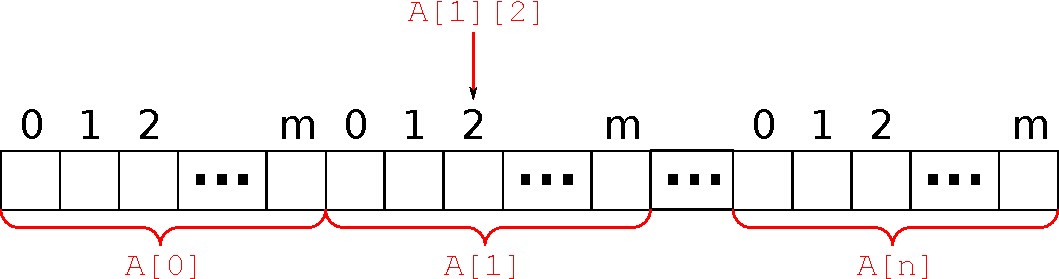
\includegraphics[width=0.85\textwidth]{matrix.pdf}
%   \end{center}
%   Mátrixok összeadása: $(A+B)[i,j] = A[i,j] + B[i,j]$, ahol $A$ és $B$ két $n\times m$ méretű mátrix.\\
% \end{frame}

% %25
% \begin{frame}{Mátrixok}
%   \begin{exampleblock}{\textattachfile{mtxOsszead1.c}{mtxOsszead1.c}}
%     \scriptsize
%     \lstinputlisting[style=c,linerange={4-20},numbers=left,firstnumber=4]{mtxOsszead1.c}
%   \end{exampleblock}
% \end{frame}

% %26
% \begin{frame}{Mátrixok}
%   \scriptsize
%   \begin{exampleblock}{\textattachfile{mtxOsszead1.c}{mtxOsszead1.c}}
%     \scriptsize
%     \lstinputlisting[style=c,linerange={21-40},numbers=left,firstnumber=21]{mtxOsszead1.c}
%   \end{exampleblock}
% \end{frame}

% %27
% \begin{frame}[fragile]{Mátrixok}
%   \begin{block}{Kimenet}
%     \begin{verbatim}
% 11 12 13 14   33 49 36 12   44 61 49 26 
% 21 22 23 24 + 20 45 24 18 = 41 67 47 42 
% 31 32 33 34   19 10 11 42   50 42 44 76
% \end{verbatim}
%   \end{block}
%   \vfill
%   Hogyan adható át egy mátrix függvénynek?\\
%   \begin{exampleblock}{OK \checkmark}
%     \texttt{void fv(int t[SOROK][OSZLOPOK]) \{ //...\\
%     void fv(int t[][OSZLOPOK]) \{ //...\\
%     void fv(int (*t)[OSZLOPOK]) \{ //...}
%   \end{exampleblock}
%   \begin{alertblock}{Hiba X -- Ez mutatótömb, nem mátrix!}
%     \texttt{void fv(int *t[OSZLOPOK]) \{ //...}
%   \end{alertblock}
% \end{frame}

% %28
% \begin{frame}{Mátrixok}
%   \begin{exampleblock}{\textattachfile{mtxOsszead2.c}{mtxOsszead2.c}}
%     \lstinputlisting[style=c,linerange={44-56},numbers=left,firstnumber=44]{mtxOsszead2.c}
%   \end{exampleblock}
% \end{frame}

% %29
% \begin{frame}{Mátrixok}
%   \scriptsize
%   \begin{exampleblock}{\textattachfile{mtxOsszead2.c}{mtxOsszead2.c}}
%     \scriptsize
%     \lstinputlisting[style=c,linerange={4-23},numbers=left,firstnumber=4]{mtxOsszead2.c}
%   \end{exampleblock}
% \end{frame}

% %30
% \begin{frame}{Mátrixok}
%   \scriptsize
%   \begin{exampleblock}{\textattachfile{mtxOsszead2.c}{mtxOsszead2.c}}
%     \scriptsize
%     \lstinputlisting[style=c,linerange={25-42},numbers=left,firstnumber=25]{mtxOsszead2.c}
%   \end{exampleblock}
% \end{frame}

% %31
% \begin{frame}{Mátrixok}
%   \begin{columns}[T]
%     \column{.5\textwidth}
%       Probléma:
%       \begin{itemize}
%         \item[] rugalmatlan függvények, mert az oszlopok száma rögzített
%       \end{itemize}
%       \vfill
%       Megoldás:
%       \begin{itemize}
%         \item hozzunk létre dinamikusan vektorokat (pl. \texttt{int*}-gal címezhetők), majd 
%         \item ezek címeit tároljuk egy újabb, dinamikus vektorban (\texttt{int**}, mutatótömb)!
%       \end{itemize}
%     \column{.5\textwidth}
%       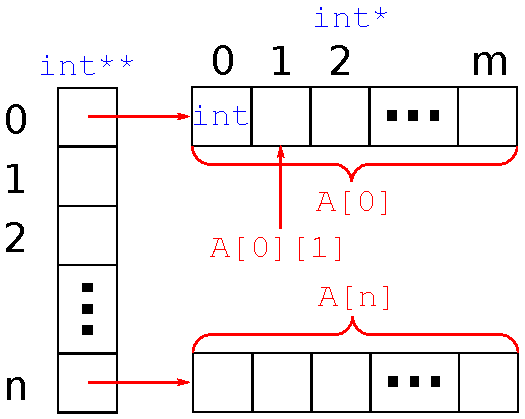
\includegraphics[width=\textwidth]{matrix2.pdf}
%   \end{columns}
% \end{frame}

% %32
% \begin{frame}{Mátrixok}
%   \footnotesize
%   \begin{exampleblock}{\textattachfile{mtxOsszead3.c}{mtxOsszead3.c}}
%     \lstinputlisting[style=c,linerange={55-70},numbers=left,firstnumber=55]{mtxOsszead3.c}
%   \end{exampleblock}
% \end{frame}

% %33
% \begin{frame}{Mátrixok}
%   \begin{exampleblock}{\textattachfile{mtxOsszead3.c}{mtxOsszead3.c}}
%     \footnotesize
%     \lstinputlisting[style=c,linerange={5-19},numbers=left,firstnumber=5]{mtxOsszead3.c}
%   \end{exampleblock}
% \end{frame}

% %34
% \begin{frame}{Mátrixok}
%   \begin{exampleblock}{\textattachfile{mtxOsszead3.c}{mtxOsszead3.c}}
%     \footnotesize
%     \lstinputlisting[style=c,linerange={21-28},numbers=left,firstnumber=21]{mtxOsszead3.c}
%     \lstinputlisting[style=c,linerange={48-53},numbers=left,firstnumber=49]{mtxOsszead3.c}
%   \end{exampleblock}
% \end{frame}

% %35
% \begin{frame}{Mátrixok}
%   Alternatív megoldás:
%   \begin{itemize}
%     \item utánozzuk a ``statikus'' tömbök memóriabeli szerkezetét, azaz
%     \item valójában vektornak foglalunk helyet, és erre képezzük le a mátrix elemeit
%   \end{itemize}
%   \begin{center}
%     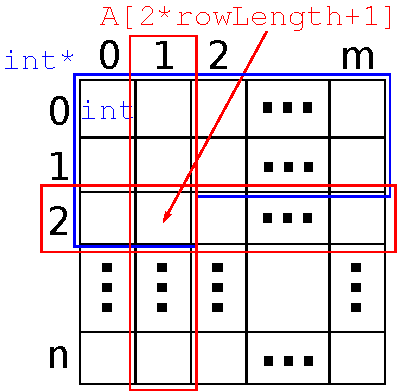
\includegraphics[scale=0.6]{matrix3.pdf}
%   \end{center}
% \end{frame}

% %36
% \begin{frame}{Mátrixok}
%   \footnotesize
%   \begin{exampleblock}{\textattachfile{mtxOsszead4.c}{mtxOsszead4.c}}
%     \lstinputlisting[style=c,linerange={44-59},numbers=left,firstnumber=44]{mtxOsszead4.c}
%   \end{exampleblock}
% \end{frame}

% %37
% \begin{frame}{Mátrixok}
%   \scriptsize
%   \begin{exampleblock}{\textattachfile{mtxOsszead4.c}{mtxOsszead4.c}}
%     \lstinputlisting[style=c,linerange={5-24},numbers=left,firstnumber=5]{mtxOsszead4.c}
%   \end{exampleblock}
% \end{frame}

\end{document}
